%! TEX root = ./main.tex

\section{Sonstiges}
\subsection{Erwartungswert}
\begin{itemize}
    \ides{Gegeben:} EW von $f(x,y) =
        \begin{cases}
            \frac{1}{2} \quad 0 \le x \le y \le 2\\
            0 \quad \text{else}
        \end{cases}$
        \ides{Gesucht:}
        $E[XY] = \int_0^2 \int_0^y \frac{1}{2} x y \ \mathrm{d}x \mathrm{d}y = \int_0^2 \left. \frac{1}{4} x^2 y \right|_0^y = \int_0^2 \frac{1}{4} y^3 \ \mathrm{d}y = \left. \frac{1}{16} y^4 \right|_0^2 = 1$
\end{itemize}

\subsection{Umformungen}
\begin{itemize}
    \item $P[|X - \mu| \le 1] = P[-1 \le X - \mu \le 1] = P[-1 + \mu \le X \le 1 + \mu] = P[X \le 1 + \mu] - P[X \le -1 + \mu]$
    \item $\frac{1}{n} \sum_{i=1}^{n} (X_i - \overline X_n)^2 = \frac{1}{n} \sum_{i=1}^n X_i^2 - (\overline X_n)^2$
    \item 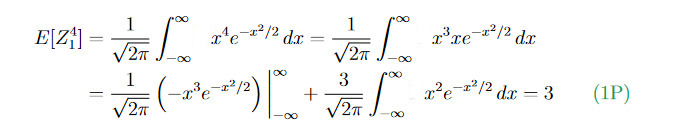
\includegraphics[width=\linewidth]{./Figures/Umformung.jpg}
\end{itemize}

\subsection{Likelihood Quotient}
\begin{itemize}
    \item
        \begin{itemize}
            \ides{Gegeben:}
                \begin{align*}
                    L(x_1, \dots, x_n;\vartheta) &= \Pi_{i=1}^n p_X(x_i;\vartheta)\\
                                                 &= \vartheta^{\sum_{i=1}^n x_i}(1 - \vartheta)^{n - \sum_{i=1}^n x_i}
                \end{align*}
            \ides{Gesucht:}
                \begin{align*}
                    R(x_1, \dots, x_n; \vartheta_0, \vartheta_A) &= \frac{L(x_1, \dots, x_n; \vartheta_A}{L(x_1, \dots, x_n; \vartheta_0}\\
                                                                 &= \left( \frac{\vartheta_A}{\vartheta_0} \right)^{\sum_{i=1}^n x_i} \left(\frac{1 - \vartheta_A}{1 - \vartheta_0} \right)^{n - \sum_{i = 1}^n x_i}\\
                                                                 &= \left( \frac{\vartheta_A (1 - \vartheta_0)}{\vartheta_0 (1 - \vartheta_A)} \right)^{\sum_{i=1}^n x_i} \left(\frac{1 - \vartheta_A}{1 - \vartheta_0} \right)^n
                \end{align*}
                    \begin{itemize}
                        \item Sei $\vartheta_0 = \frac{1}{2}, \vartheta_A \ge \frac{1}{2}$, so ist $R$ gross, falls $\sum_{i=1}^n x_i$ gross ist $\implies T := \sum_{i=1}^n X_i = S_n$
                    \end{itemize}
        \end{itemize}
    \item
        \begin{itemize}
            \ides{Gegeben:}
                \begin{align*}
                    L(x_1, \dots, x_n;\vartheta) &= \Pi_{i=1}^n f_X(x_i;\vartheta)\\
                                                 &= (2 \pi \sigma^2)^{\frac{-n}{2}} \exp \left(- \frac{1}{2 \sigma^2} \sum_{i=1}^n (x_i -\vartheta)^2 \right)
                \end{align*}
            \ides{Gesucht:}
                \begin{align*}
                    R(x_1, \dots, x_n; \vartheta_0, \vartheta_A) &= \frac{L(x_1, \dots, x_n; \vartheta_A}{L(x_1, \dots, x_n; \vartheta_0}\\
                                                                 &= \exp \left( -\frac{1}{2 \sigma^2} \left( \sum_{i=1}^n (x_i - \vartheta_A)^2 - \sum_{i=1}^n (x_i - \vartheta_0)^2 \right) \right)\\
                                                                 &= \text{const.}(\sigma, \vartheta_0, \vartheta_A) \exp \left( \frac{1}{2 \sigma^2} (\vartheta_A - \vartheta_0) \sum_{i=1}^n x_i \right)\\
                \end{align*}
            \item Für $\vartheta_0, \vartheta_A$ beliebig, $R$ ist gross wenn $(\vartheta_A - \vartheta_0) \sum_{i=1}^n x_i$ gross ist $\implies T := \sum_{i=1}^n X_i$
        \end{itemize}
\end{itemize}

\subsection{Likelihood Schätzer}
\begin{itemize}
    \ides{Gesucht:} Maximum-Likelihood Schätzer für $\lambda$ für $X_1, \dots, X_n$, i.i.d. $X_i \sim \text{Poisson}(\lambda)$ ist $T = \frac{1}{n} \sum_{i=1}^n X_i$
    \ides{Gesucht:} Maximum-Likelihood Schätzer für $p$ für $X_1, \dots, X_n$, i.i.d. $X_i \sim \text{Be}(p)$ ist $T = \frac{1}{n} \sum_{i=1}^n X_i$
\end{itemize}

\subsection{Mehrere ZV}
\begin{itemize}
    \ides{Gegeben:} $Z \sim \text{Exp}(\lambda), Z \sim \text{Exp}(\mu)$
\ides{Gesucht:} $P[Z > Y] = \int \int_{\{(y,z) \in \R^2 \mid z > y \}} \lambda e^{-\lambda y} \mu e^{-\mu z} \mathrm{d}z \mathrm{d}y = \int_0^\infty \lambda e^{\lambda y} \int_y^\infty \mu e^{-\mu z} \mathrm{d}z \mathrm{d}y = \int_0^\infty \lambda e^{-\lambda y} e^{-\mu y} \mathrm{d}y = \frac{\lambda}{\lambda + \mu}$
\end{itemize}

\subsection{Proof Gedächnislos}
Beweise: $Y \sim Exp(p) \iff P[Y > s] = P[Y > s + t \mid Y > t], \quad s,t \in \R_+$:
\\ 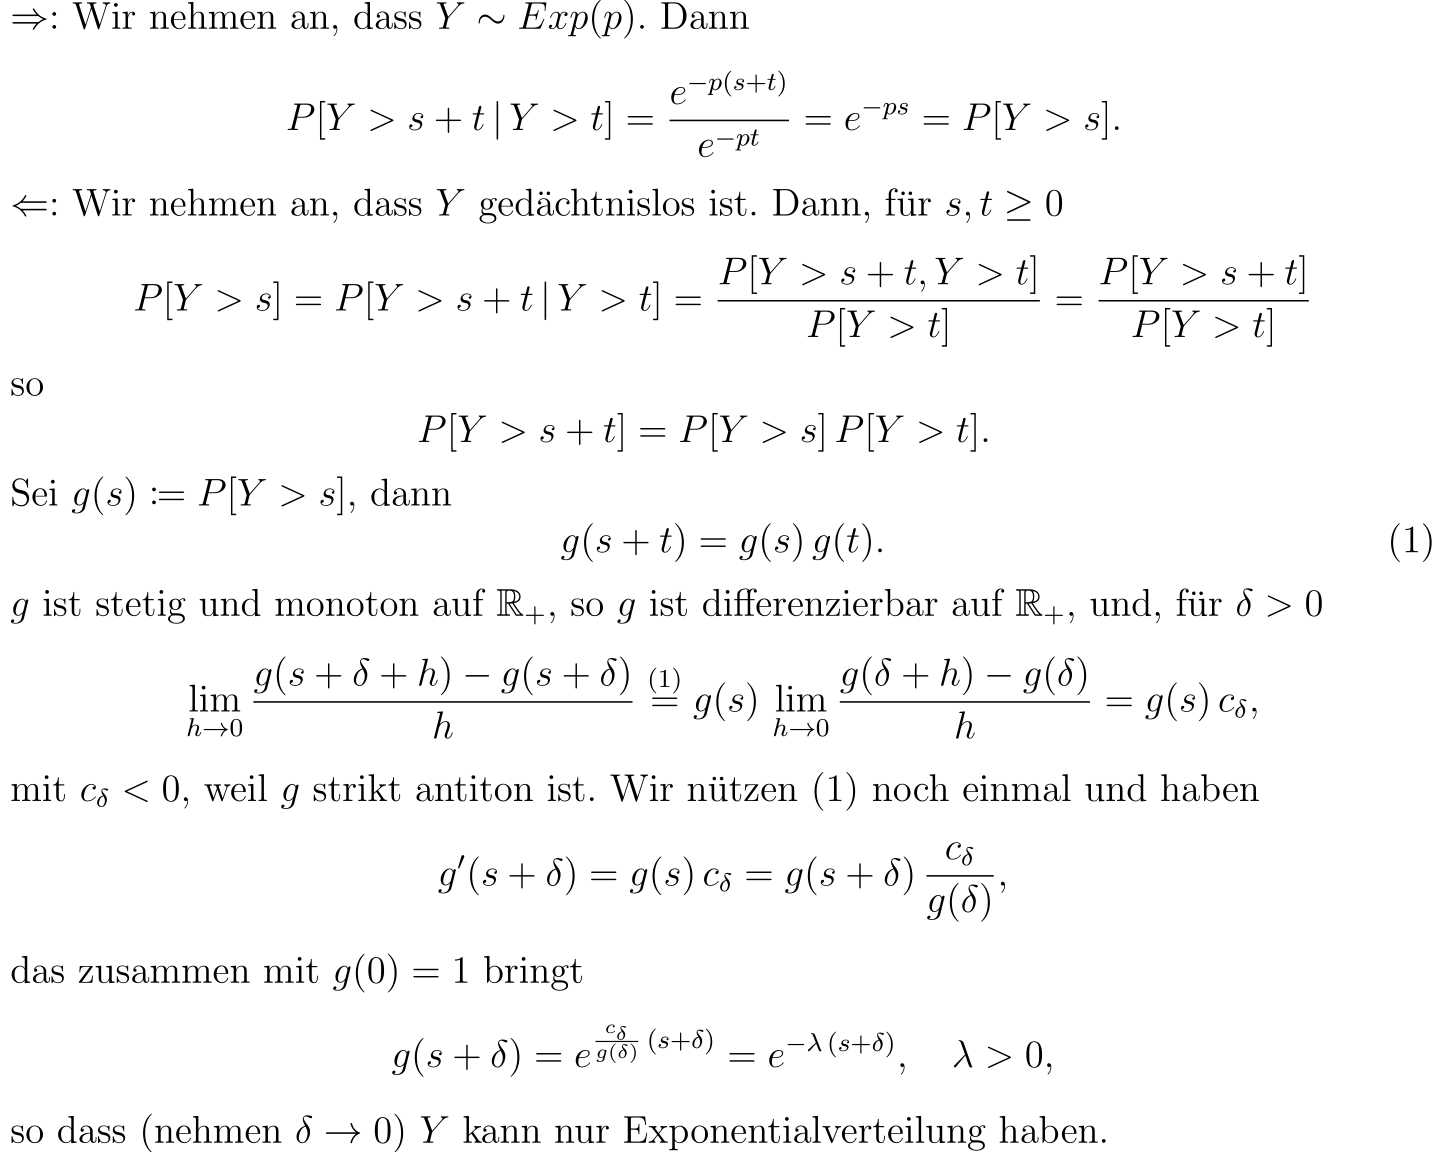
\includegraphics[width=\linewidth]{./Figures/proof_Gedaechnislos.png}

\subsection{Hypergeometrische Verteilung}
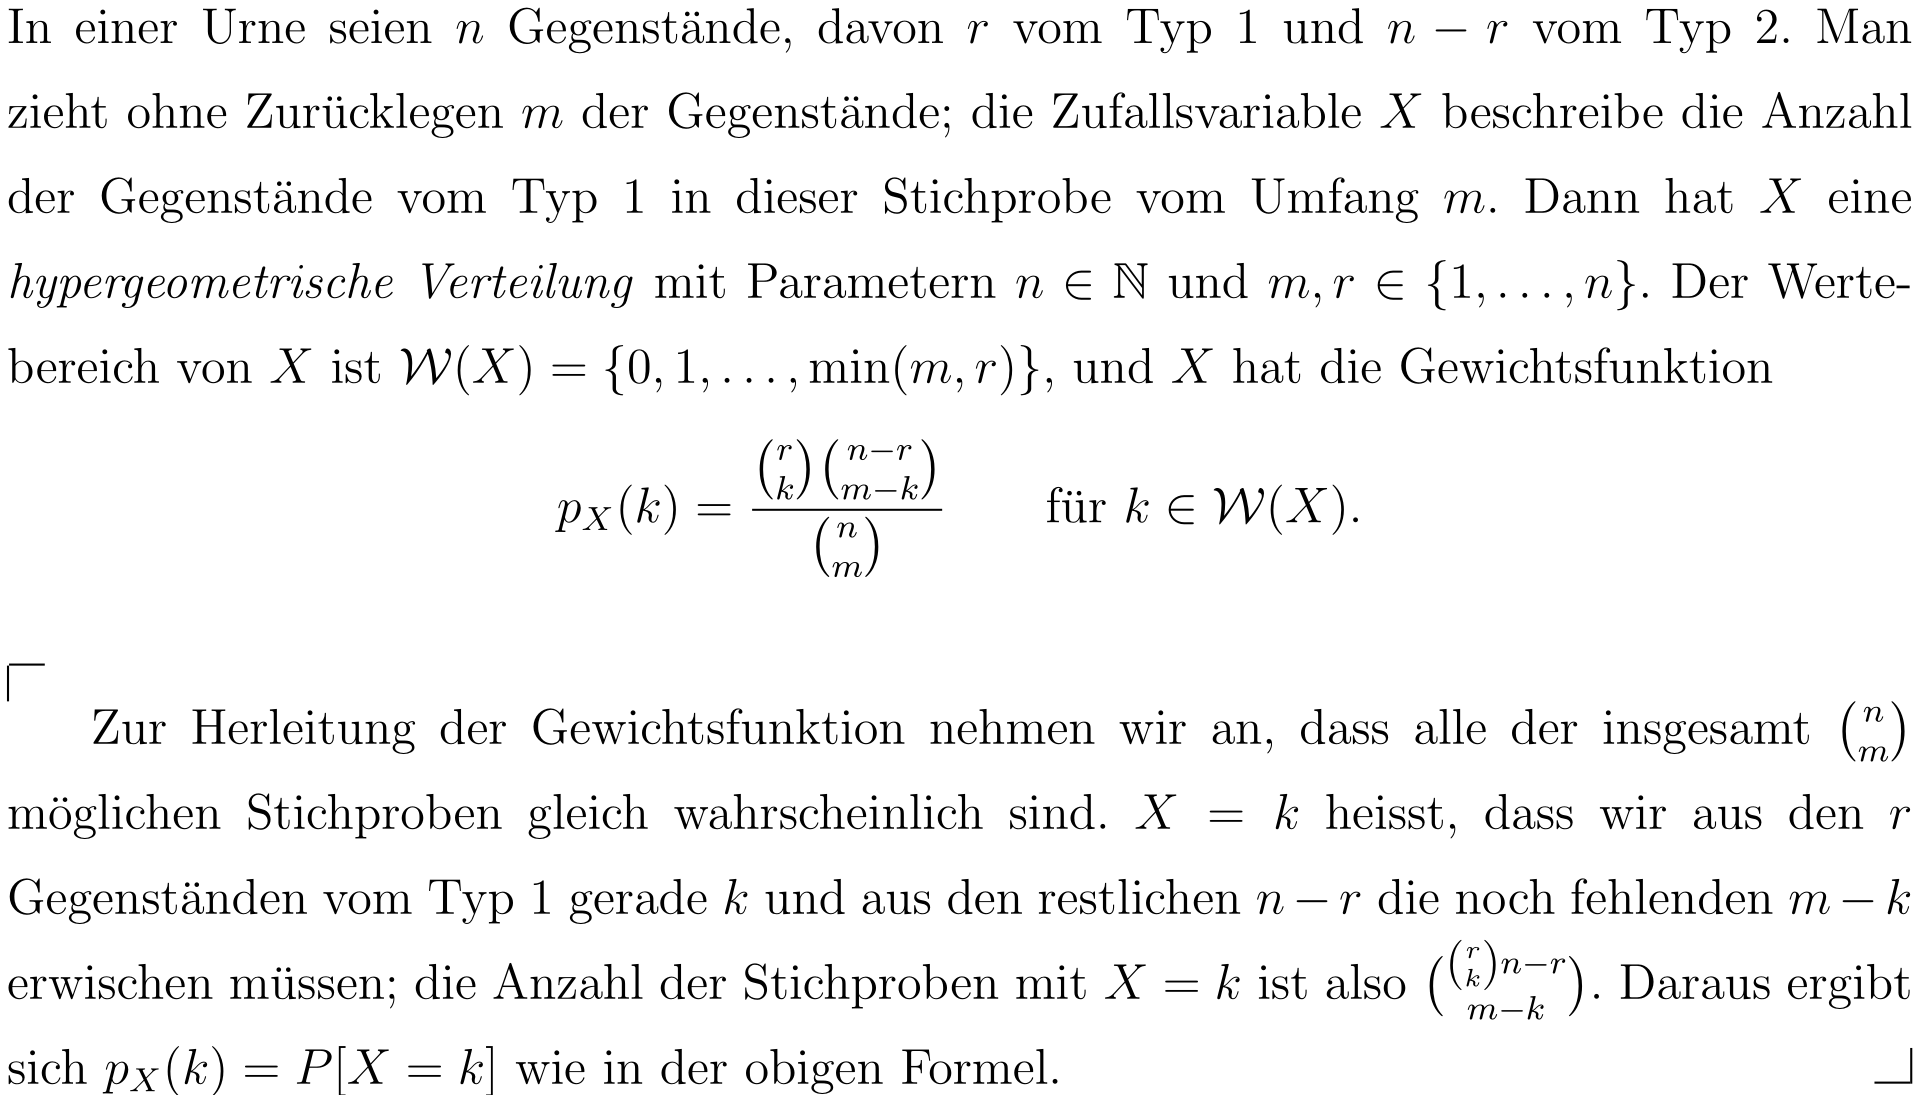
\includegraphics[width=\linewidth]{./Figures/Hypergeometrische_Verteilung.png}

\subsection{Momenteschätzer}
\begin{itemize}
    \item Für ein Experiment mit $n=5$ unf $f_T(t) = C^2 e^{-Ct} 1_{[0 \le t]}$, bestimme den Momenteschätzer:
        \\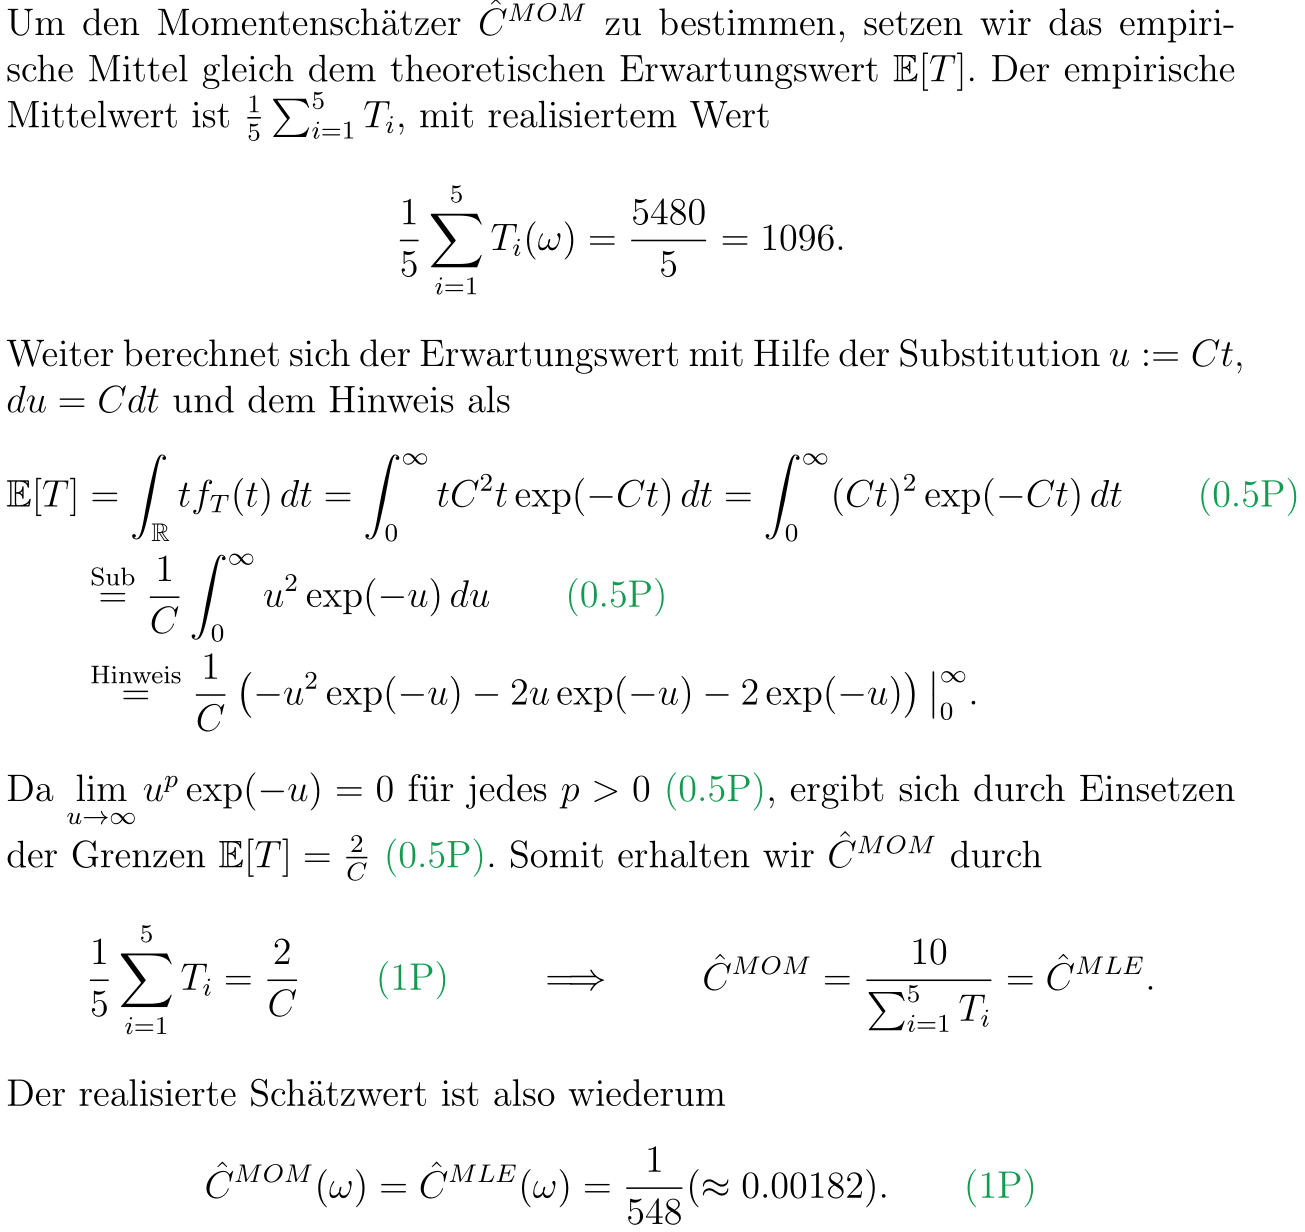
\includegraphics[width=\linewidth]{./Figures/Momente_Schaetzer.png}
    \item More MM:
        \\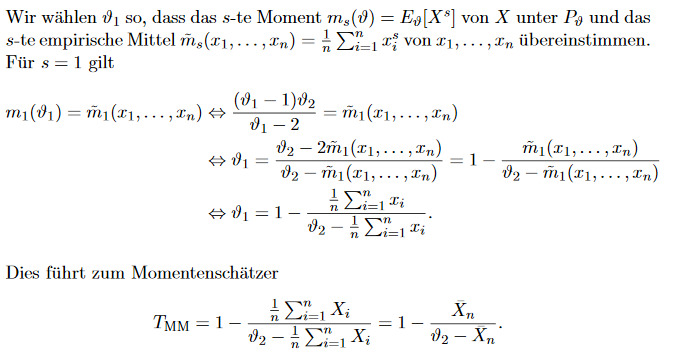
\includegraphics[width=\linewidth]{./Figures/MomenteschaetzerII.jpg}
\end{itemize}

\subsection{Test Nicht Normalverteilt}
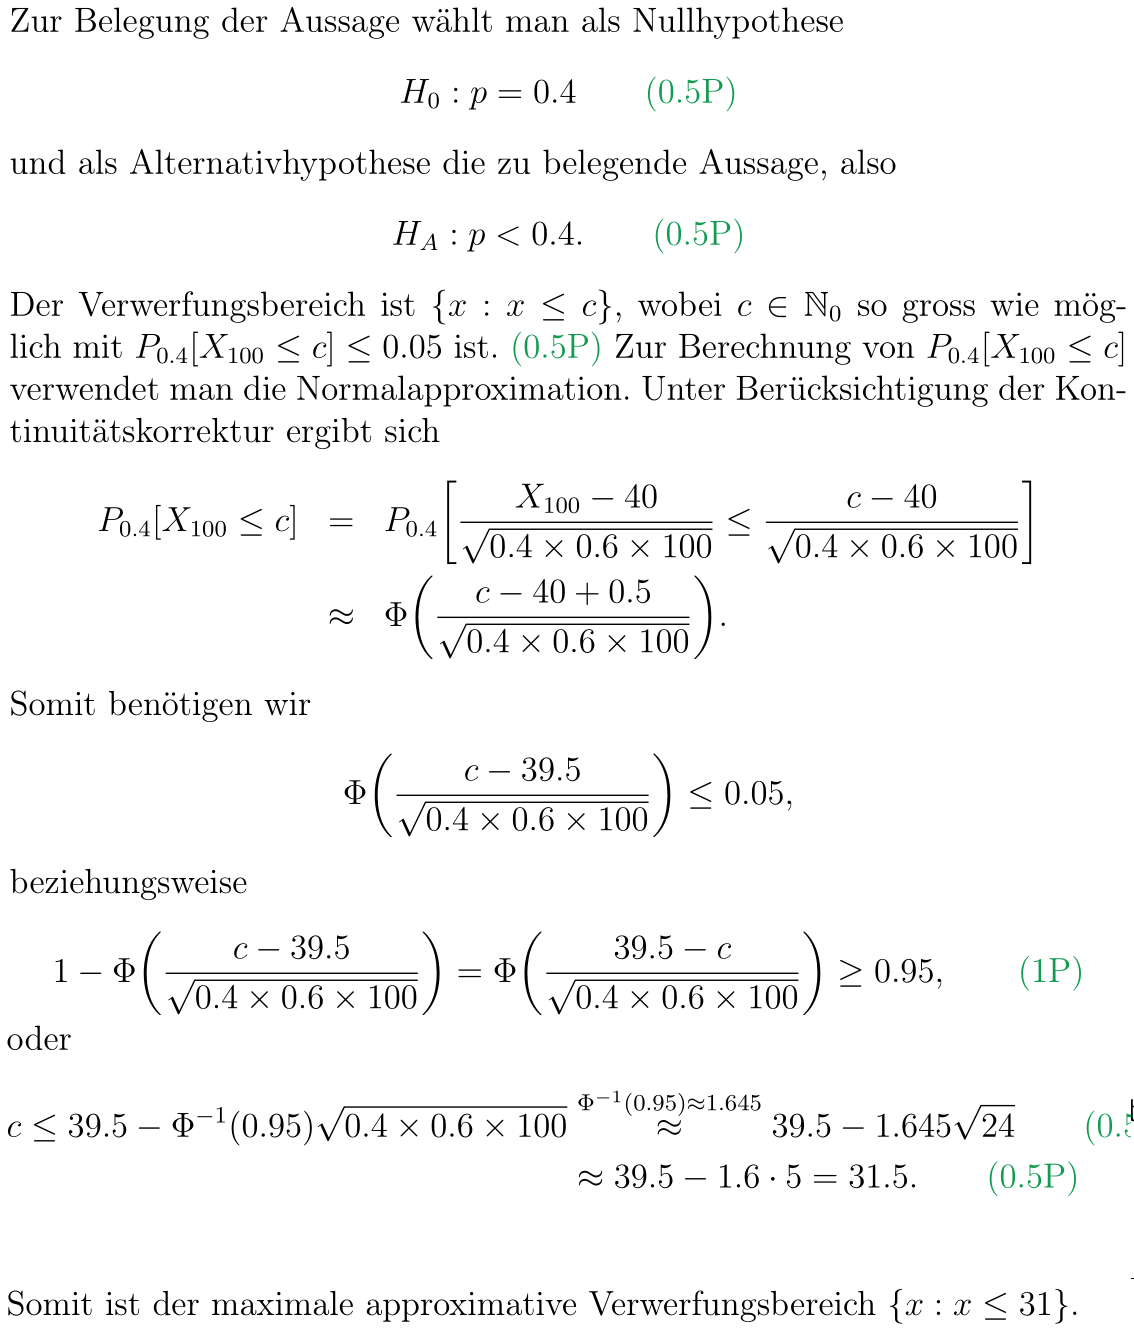
\includegraphics[width=\linewidth]{./Figures/Test_Nicht_Normalverteilt.png}

\subsection{MinStuff}
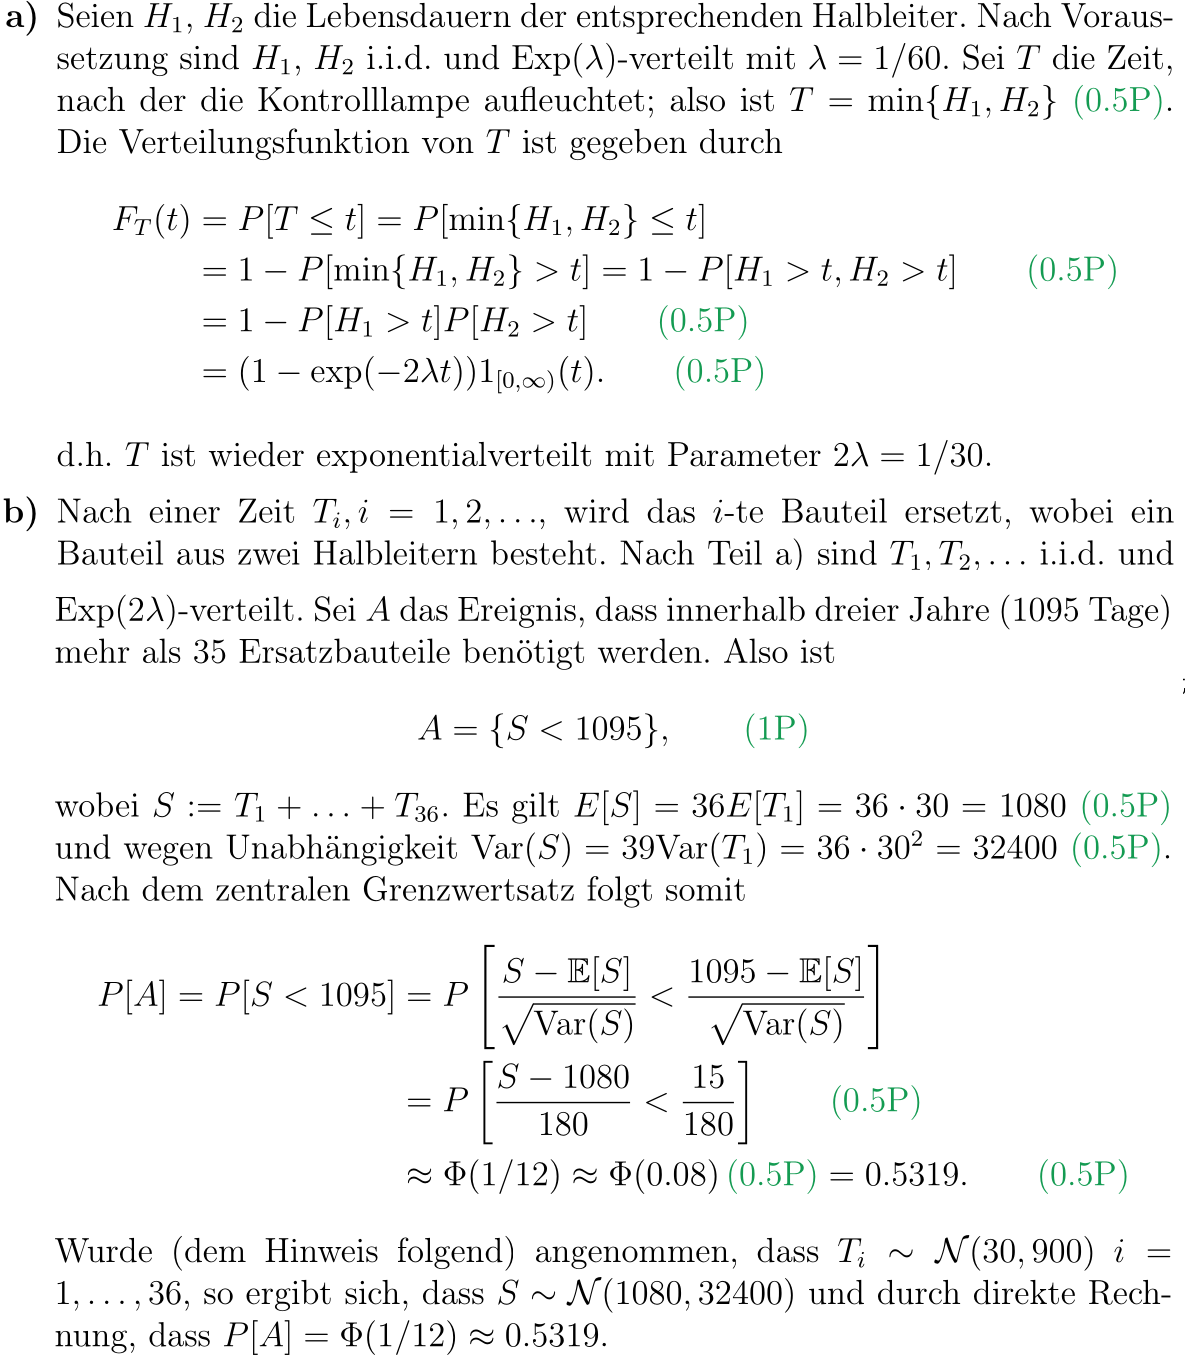
\includegraphics[width=\linewidth]{./Figures/ExampleMinStuff.png}

\subsection{$\chi$ Verteilung}
Für $Y = \sum_{k=1}^v Z_k^2, \quad Z_i \sim \mc{N}(0,1)$ i.i.d. find $E[Y], Var[Y]$:
\\ 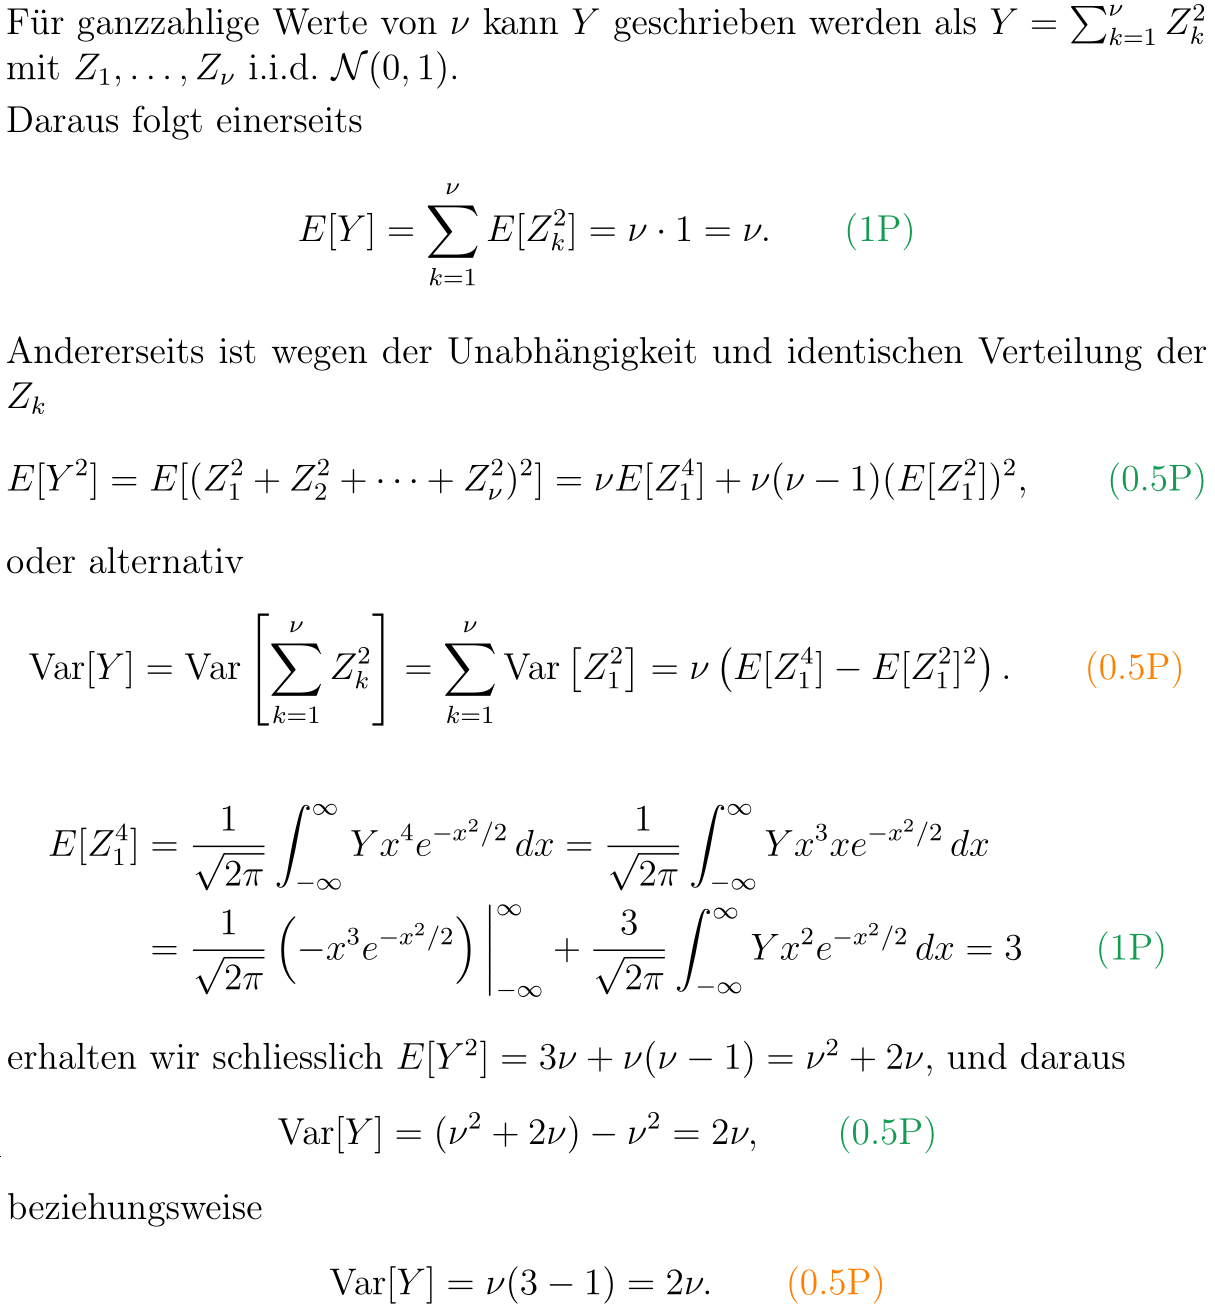
\includegraphics[width=\linewidth]{./Figures/chi_verteilung.png}

\subsection{Grenzwert Überschreitung}
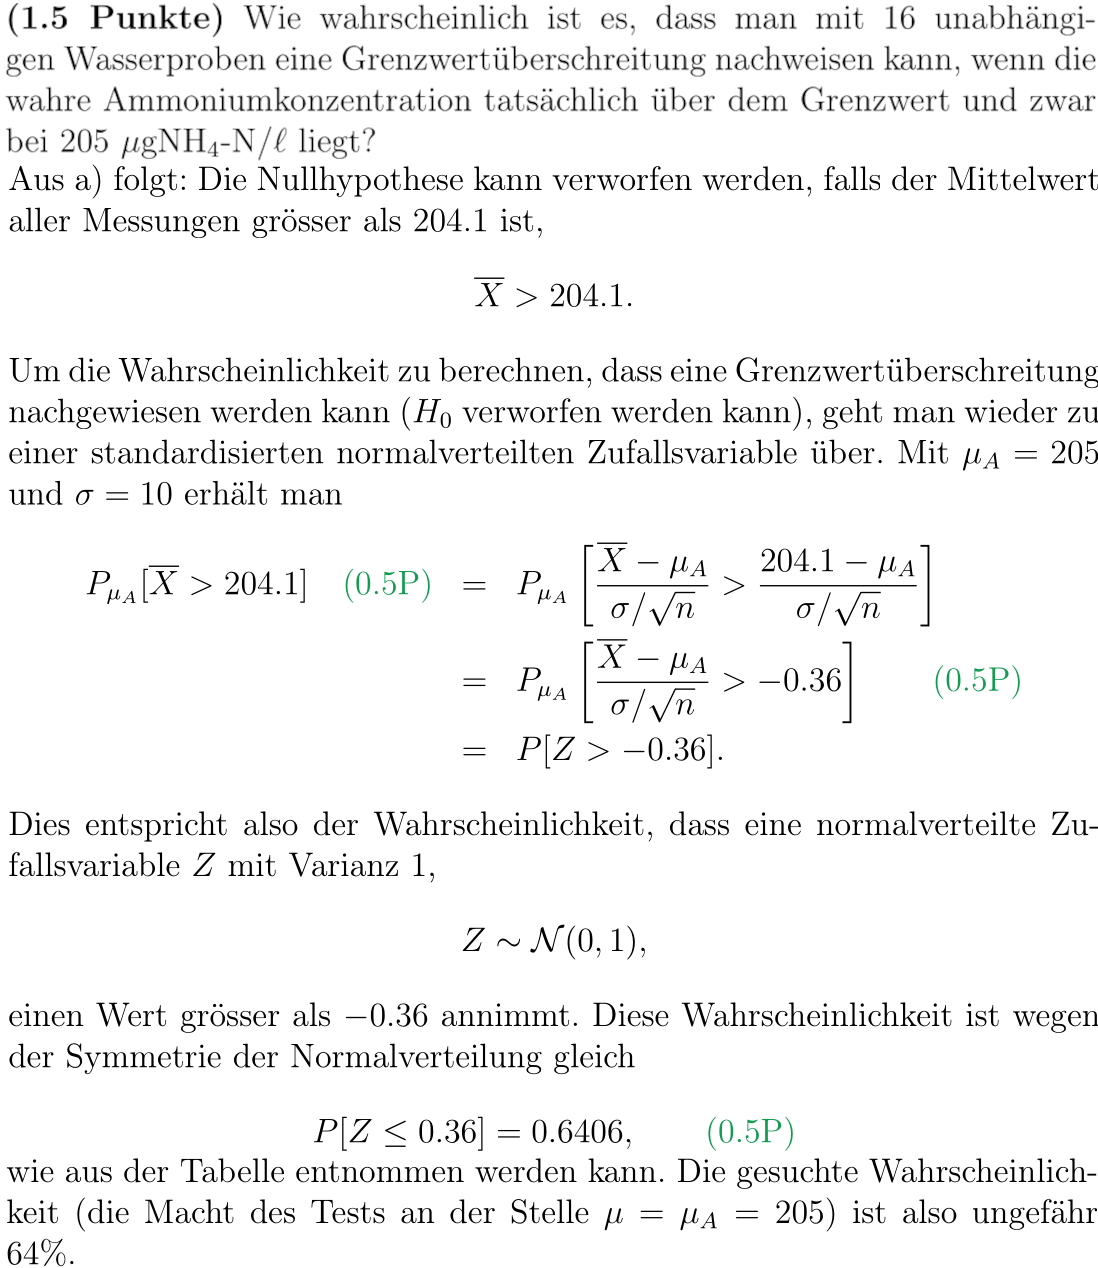
\includegraphics[width=\linewidth]{./Figures/Test_Ueberschreitung.png}

\subsection{Gemeinsame Dichte und Randdichte}
$P \sim \text{Uniform}(0,1), H|P \sim \text{Uniform}(0,P)$, finde:
\begin{itemize*}
    \item Gemeinsame Dichte
    \\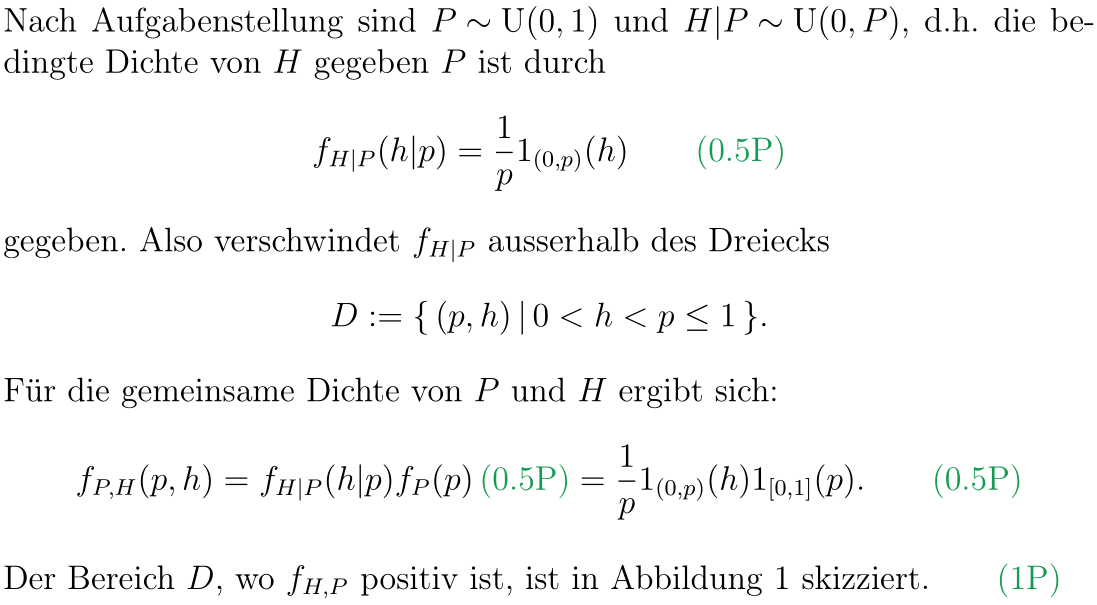
\includegraphics[width=\linewidth]{./Figures/Gemeinsame_Dichte_Randdichte_A.png}
    \item Randdichte von $H$
    \\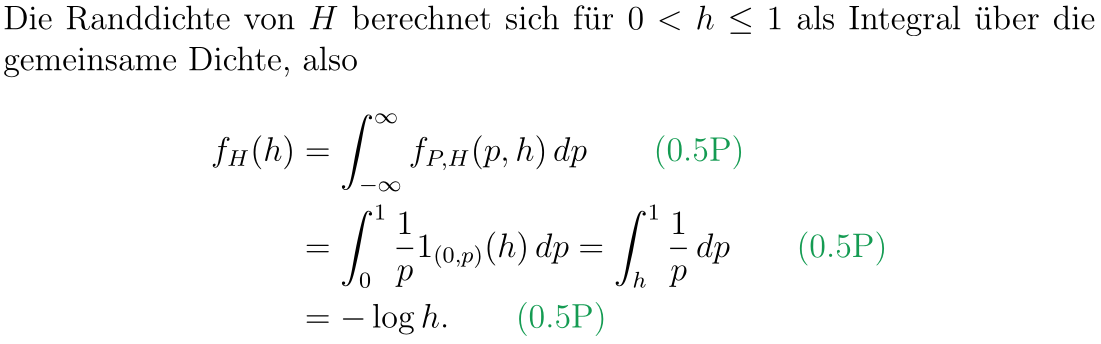
\includegraphics[width=\linewidth]{./Figures/Gemeinsame_Dichte_Randdichte_B.png}
    \item $E[H]$
    \\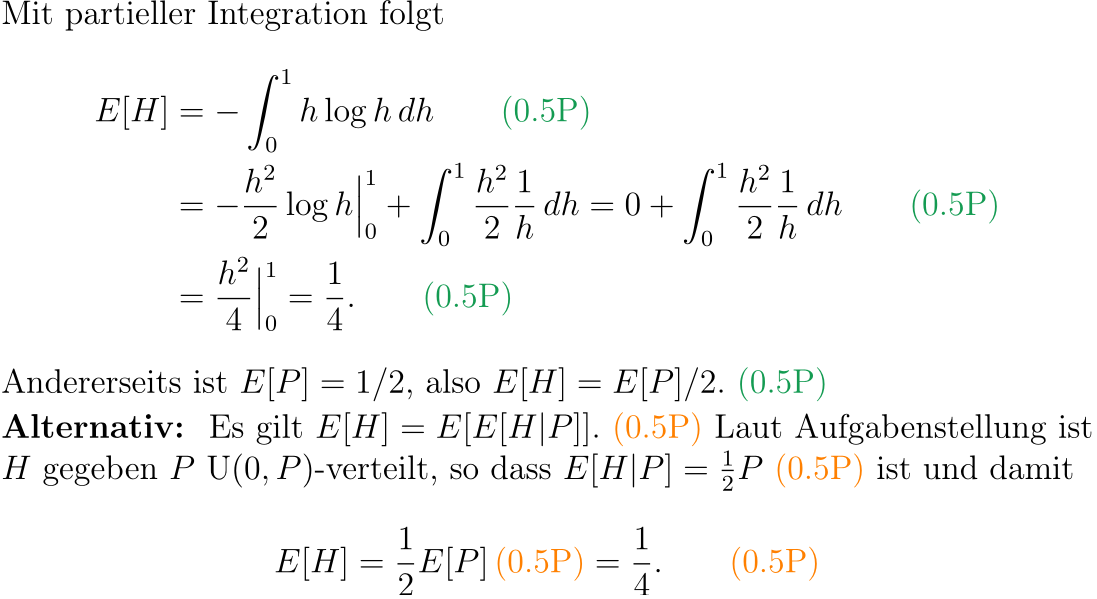
\includegraphics[width=\linewidth]{./Figures/Gemeinsame_Dichte_Randdichte_C.png}
\end{itemize*}
